
\section{Introduction}

gptools is a framework that empowers teams, including non-developers, to create and use AI-enhanced scripts to support their workflows. gptools provides support for creating, understanding, and maintaining complex collections of documents such as software repositories, project management, etc. Our framework leverages foundation models (specifically LLMs) to enable a new kind of scripting that combines traditional code and natural language.

\section{Key Elements of gptools}

The key elements of the gptools framework are gpspecs and gptools. gpspecs are natural language documents that describe specific user tasks to accomplish. gptools are general scripts that combine traditional software and natural language prompts and rely on an LLM to generate results. We execute gptools in the context of a gpspec to achieve a result. By separating these two abstractions, we allow gptools to be authored, maintained, and updated independently of the gpspecs that use them. The gptools framework includes an execution engine to execute a gptool and an IDE extension to VS Code to support user interaction with the gptool.

\tikzstyle{block} = [rectangle, draw, text width=5em, text centered, rounded corners, minimum height=4em]
\tikzstyle{arrow} = [thick,->,>=stealth]

\begin{figure}[h]
\centering
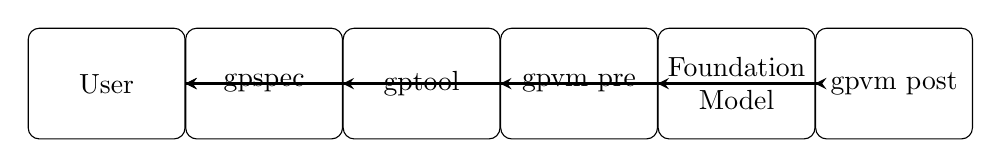
\begin{tikzpicture}[node distance=2cm]
\node (user) [block] {User};
\node (gpspec) [block, right of=user] {gpspec};
\node (gptool) [block, right of=gpspec] {gptool};
\node (gpvmPre) [block, right of=gptool] {gpvm pre};
\node (foundationModel) [block, right of=gpvmPre] {Foundation Model};
\node (gpvmPost) [block, right of=foundationModel] {gpvm post};

\draw [arrow] (user) -- (gpspec);
\draw [arrow] (gpspec) -- (gptool);
\draw [arrow] (gptool) -- (gpvmPre);
\draw [arrow] (gpvmPre) -- (foundationModel);
\draw [arrow] (foundationModel) -- (gpvmPost);
\draw [arrow] (gpvmPost) -- (user);
\end{tikzpicture}
\caption{Workflow of gptools}
\end{figure}


\section{Complex Artifacts Require Complex Workflows}

Software development is a complex process that requires the coordination of many different activities. Historically, software development has been a highly manual process, with developers using a variety of tools to create and maintain the artifacts that comprise a software system. Over time abstractions have been developed to help manage the complexity of software development. Important examples include: Unix utilities and pipes, makefiles, build scripts, etc. Modern software development includes many automated processes as well as manual processes such as code review, design review, bug triage, etc.

\section{Foundation Models Create New Opportunities}

The recent development of foundation models (aka LLMs) have created new opportunities for automating complex workflows. AI has important advantages over traditional software: AI models can perform tasks normal software cannot and AI models can be instructed using natural language, allowing non-programmers to use them. AI models also have disadvantages: AI models are not perfect, and can make mistakes and AI models are not transparent, and it is difficult to understand why they make the decisions they do. AI models are best used to augment human workflows, not replace them.

\section{gptools - a Framework for AI-Enhanced Workflows}

Vision: empower teams, including non-developers, to use AI-enhanced scripts to support their efforts to create, understand, and maintain complex artifacts. Goals: support tool abstraction, modularity, reuse, but at the same time empower non-developers to author, maintain, and update AI-enhanced scripts. Approach: Foundation models enable a new kind of scripting that allows script writers to achieve both greater functionality and greater ease of use. We separate scripts into two related parts: a generic reusable \textit{gptool} and a natural language \textit{gpspec} that instantiates the gptool in a particular context.

\section{gptool: A New Kind of Script}

A gptool is a script with the following components: A header that contains metadata related to the execution of the script (e.g., information about what LLM model to use, etc.), a natural language prompt intended to be processed by a foundation model, an environment context that augments the natural language with additional data/information, and programming language constructs that are used to programmatically manipulate both inputs and outputs.

\section{gpspec: Natural Language to Invoke a gptool}

Just as a chat enables a user to interact with an AI model, a gpspec is a natural language markdown document that defines a context in which to invoke a gptool. A gpspec is a standard markdown file, with the following additional elements: Links to context elements that define the context in which a particular gptool is to be invoked. For example, a gpspec might contain links to markdown files, code files, etc. Natural language describing the specific task to be performed as input to a gptool. For example, the spec used to generate code would include a description of the functionality and might include a description style guidelines to observe, etc.

\section{gpvm - A Framework for Executing gpspecs and gptools}

Every system that interacts with a foundation model includes layers that transform user input into a prompt that can be processed by the foundation model, and layers that transform the output of the foundation model into a form that is useful to the user. gpvm is a runtime environment that captures the context defined by the gpspec, executes whatever code is present in the gptool, expands the gpspec and natural language of the gptool into a prompt that can be processed by the foundation model, sends the results to the AI model, and processes the results on return to update the user context (which might include creating files, updating files, generating user feedback, etc.).

\section{gptools Extension to VS Code}

We believe that human oversight of AI models is essential to their effective use. To support this, we have created a VS Code extension that allows a user to interact with a gpspec and gptool in a natural way. The extension provides the following capabilities: A command palette that allows a user to select a gptool to invoke in the context of a given gpspec file, a token management system that supports connecting with the AI model of interest, an invocation of the gpvm to process the user input and generate results, a user interface that allows the user to interact with the AI model to refine the results, and a gptool trace viewing mechanism that allows users to understand how the AI model was used to generate the results.

\section{Implications of gptools}

The existence of powerful programming tools based on AI that are usable by non-developers is transformative. Just as the development of JavaScript enabled Web 2.0, and python enabled the creation of the current AI software ecosystem, gptools will fuel a new generation of AI-enhanced applications. We envision the creation of gptools for many different verticals, with opportunities for customization and authoring at many levels of expertise: Professional developers and architects will define collections of gptools for a given vertical just as packages are authored and maintained today, professional developers can author and maintain individual gptools, developers and non-developers can customize gptools for their particular organization or application needs, and non-developers can author and maintain gpspecs for their particular projects. Furthermore, the existence of gptools can empower non-developers to automate their workflows in ways that were previously impossible.

\section{Related Work}

gptools are related to a number of foundation model projects that automate workflows and encapsulate LLM actions in software artifacts. We describe some of these projects below:

\subsection{AI Tools for Developers}

\begin{itemize}
\item GitHub Copilot is a VS Code extension that uses the Codex LLM to suggest code completions based on the context of the current file. Copilot provides LLM support for writing code but does not currently have an extensibility model or a way to create, maintain and apply collections of AI-enhanced scripts.
\item codeplan is a task-agnostic framework that frames repository-level coding as a planning problem, synthesizing a multi-step chain of edits where each step results in a call to an LLM on a code location with context derived from the entire repository, previous code changes, and task-specific instructions. While codeplan uses LLM prompts to generate code, it does not provide a way to create, maintain and apply collections of AI-enhanced scripts.
\end{itemize}

\subsection{LLM Automation/Orchestration Frameworks}

\begin{itemize}
\item autogpt is an AI agent that utilizes a large language model to drive its actions and decisions. Unlike traditional language model applications, AutoGPT does not require repeated prompting by a human and can autonomously develop and manage tasks.
\item langchain is a Python library designed to simplify the development of Natural Language Processing (NLP) applications using large language models. It provides a framework for connecting language models to other sources of data and allowing them to interact with their environment.
\item semantic kernel is an open-source SDK that allows developers to easily integrate AI services with conventional programming languages such as C\# and Python. It provides a framework for connecting language models to other sources of data, allowing them to interact with their environment and perform tasks autonomously.
\item autogen is a framework for simplifying the orchestration, optimization, and automation of large language model (LLM) workflows. It offers customizable and conversable agents that leverage LLMs while addressing their limitations by integrating with humans and tools and having conversations between multiple agents via automated chat.
\end{itemize}

gptools differ from existing AI task automation frameworks in the following ways: gptools are designed to be authored, maintained, and applied by non-developers as well as developers. gptools define a separation between the gptool and the gpspec that instantiates it, allowing for modularity, reuse, and easier understanding by non-developers. gptools do not assume task automation and provide a user experience that integrates seamlessly with VS code. The gptools UI exposes both the content and execution of each gptools to facilitate human oversight and understanding of how the AI model was used to generate the results.
    


    